\documentclass[12pt]{article}

\usepackage{fullpage}
\usepackage[top=20mm, bottom=40mm, left=10mm, right=10mm]{geometry}
\usepackage{amsmath,amsthm,amssymb}
\usepackage{lastpage}
\usepackage{enumerate}
\usepackage{fancyhdr}
\usepackage{xcolor}
\usepackage{graphicx}
\usepackage{listings}
\usepackage{hyperref}
\usepackage{answers}
\usepackage{setspace}
\usepackage{enumitem}
\usepackage{multicol}
\usepackage{mathrsfs}
\usepackage{algorithmic}
\usepackage{stmaryrd}
\usepackage[ruled,linesnumbered,vlined]{algorithm2e}
\usepackage{tikz}
\usetikzlibrary{automata, positioning}

\hypersetup{%
  colorlinks=true,
  linkcolor=blue,
  linkbordercolor={0 0 1}
}

\lstdefinestyle{Python}{
    language        = Python,
    frame           = lines, 
    basicstyle      = \footnotesize,
    keywordstyle    = \color{blue},
    stringstyle     = \color{green},
    commentstyle    = \color{red}\ttfamily
}

\setlength{\parindent}{0.0in}
\setlength{\parskip}{0.05in}

\newcommand\course{\textbf{EE 456}}   
\newcommand\name{Aishwarye Omer}     

\pagestyle{fancyplain}
\headheight 35pt
\lhead{\name\\\course{}}
\chead{\textbf{\Large Homework - 03}}
\rhead{\today}
\lfoot{}
\cfoot{}
\rfoot{\small\thepage}
\headsep 1.5em

\newlength\myindent
\setlength\myindent{2em}
\newcommand\bindent{%
  \begingroup
  \setlength{\itemindent}{\myindent}
  \addtolength{\algorithmicindent}{\myindent}
}
\newcommand\eindent{\endgroup}

\newenvironment{solution}[1][Solution]{\begin{trivlist}
\item[\hskip \labelsep {\bfseries #1}]}{\end{trivlist}}


\begin{document}

\textbf{Question: } \text{Design the state diagram for the recursive auto-associator discussed in class.}
\BlankLine
\BlankLine
\textbf{Solution: } Following image contains the state diagram for the inputs $S_i$ where $i \in \{0,1,2,...,15\}$ 
\begin{figure}[h]

	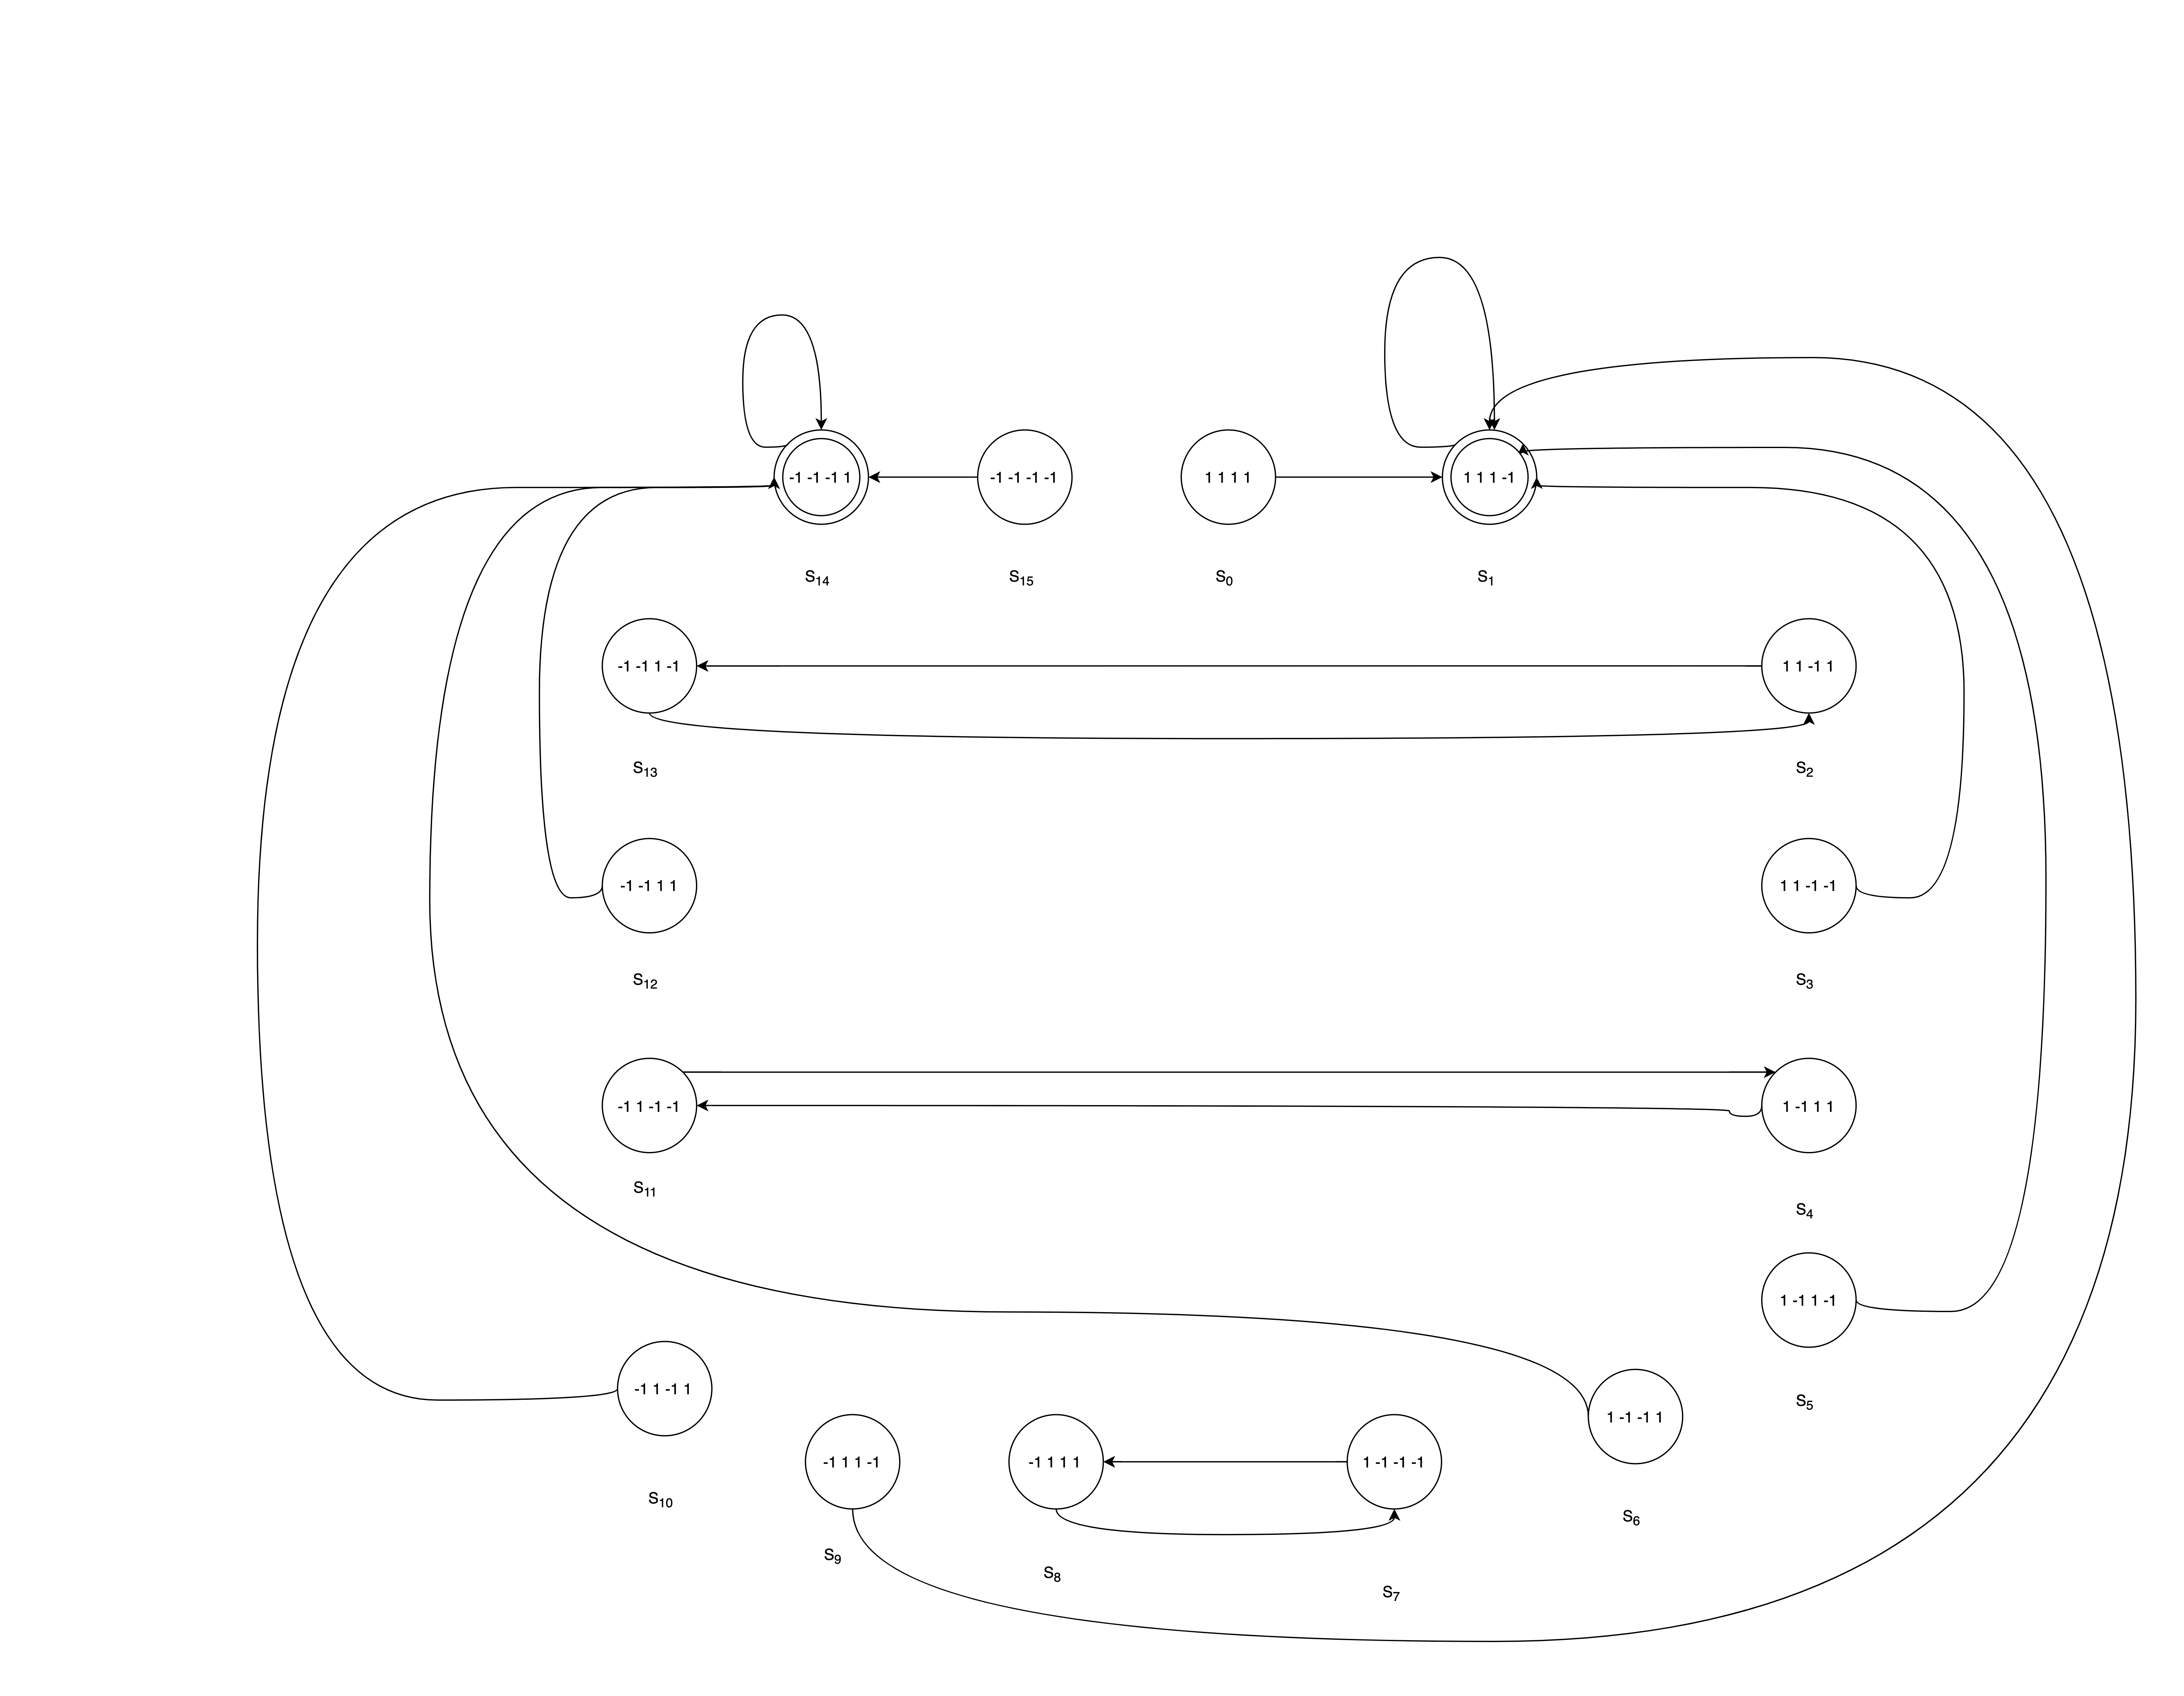
\includegraphics[width=16cm]{rec.png}
	\caption{State Diagram}
\end{figure}

The correct outputs are $S_1$ and $S_{14}$. Rest of them are incorrect outputs and oscillate between themselves.
	


\end{document}